\subsection{Užduočių diagrama}

1992 metais Ivar Jacobson apibrėžė metodologiją specifikuoti vartojimo atvejus \cite{Jacobson1992}. Jis pateikė būdą apibrėžti atvejus tiek tekstu (\ref{tab:text_use_cases_login} lentelė), tiek diagrama (\ref{img:use_cases_login} pav.). Tarp programų sistemų kūrėjų ši metodologija išpopuliarėjo kaip funkcinių reikalavimų apibrėžimo technika. \OMG{} savo specifikacijose \UML{} \cite{omgUmlFormal} ir \SysML{} \cite{OMGSysML} standartizuoja vartojimo atvejų modelį ir priskiria jį prie elgsenos apibūdinimo diagramų. 2011 metais Ivar Jacobson paskelbė užduočių modelio 2.0 versiją \cite{jacobson2011usecase}, kuri pritaikyta prie judrių metodologijų projektų įgyvendinimo.

\begin{center}
    \begin{longtable}{|p{\textwidth}|}
    \caption{Tekstinio naudojimo atvejo pavyzdys}
	\label{tab:text_use_cases_login}
	\\ \hline 
    \begin{tabular}{@{}p{3.5cm}p{12cm}}
    	\\ 
    	\textbf{ID} & NA1
    	\\ 
    	\textbf{Pavadinimas} & Registruoto naudotojo autentifikacija
    	\\ 
    \end{tabular}
    \\
    \textbf{Aktoriai}
    \begin{enumerate}
    	\item Registruotas naudotojas.
    	\item Išorinė autentifikavimosi sistema.
	\end{enumerate} 
    \\
    \textbf{Aprašas}
    
    Registruotas naudotojas autentifikuojasi sistemoje. 
    
    \\
    \textbf{Prieš sąlygos}
    \begin{enumerate}
    	\item Naudotojas nėra autentifikuotas sistemoje.
	\end{enumerate} 
    \\
    \textbf{Priežastys}
    \begin{enumerate}
    	\item Naudotojas pareikalavo būti autentifikuotas.
	\end{enumerate} 
    \\
    \textbf{Po sąlygos}
    \begin{enumerate}
    	\item Naudotojas yra autentifikuotas sistemoje.
	\end{enumerate} 
    \\
    \textbf{Pagrindinė užduočių seka}
    \begin{enumerate}
    	\item Sistema pateikia autentifikacijos variantus.
    	\item Naudotojas autentifikuojasi sistemos turimu autentifikacijos būdu.\label{seka:1_main_choose_autentification} 
		\item Sistema pateikia patvirtinimą, kad naudotojas autentifikavosi. \label{seka:1_main_success} 
	\end{enumerate}
    \\
    \textbf{Alternatyvios užduočių sekos}
    \newlist{seka}{enumerate}{5}
	\setlist[seka]{label*=\arabic*.,leftmargin=2em}
	\setlist[seka,1]{label=\ref{seka:1_main_choose_autentification}.\arabic*.,leftmargin=2em}
	\begin{seka} 
  		\item Naudotojas autentifikuojasi išorine autentifikavimosi sistema.
	\end{seka}   
    \\ 
    \textbf{Išimtinės užduočių sekos}
	\newlist{seka}{enumerate}{5}
	\setlist[seka]{label*=\arabic*.,leftmargin=2em}
	\setlist[seka,1]{label=*.\arabic*.,leftmargin=2em}
	\begin{seka} 
  		\item Naudotojas atsisako autentifikuotis.
  		\begin{seka}
  			\item Naudotojas pateikia atsisakymą autentifikuotis.
  			\item Sistema nebereikalauja autentifikacijos duomenų.
  		\end{seka}
	\end{seka}    
	\setlist[seka,1]{label=\ref{seka:1_main_success}.\arabic*.,leftmargin=2em}
	\begin{seka} 
  		\item Naudotojo pateikti duomenys neautentifikuoja jo.
  		\begin{seka}
  			\item Sistema naudotojui pateikia pranešimą apie tai, kad jo pateikti duomenys neautentifikuoja registruoto sistemos naudotojo.
  		\end{seka}
	\end{seka}
    \\ 
    \\ \hline 
    \end{longtable}
\end{center} 
Lentelėje nr.\ref{tab:text_use_cases_login} pavaizduotas autentifikavimosi sistemoje  tekstinio naudojimo atvejo pavyzdys. Naudojimo atvejai paprastai turi identifikacijos numerį pagal kurį nurodomi reikalavimų specifikacijoje. Taip pat pavadinimą, kad būtų patogiau apie jį kalbėti. Išvardinami aktoriai dalyvaujantys vykdyme. Naudojimo atvejis trumpai ir aiškiai aprašomas. Nurodomos kokios aktualios sąlygos būna prieš vykdant, kas įtakojo vykdymą ir rezultatai. Tuomet išvardinamos užduotys reikalingos pasiekti rezultatui. Jeigu naudojimo atvejis gali būti įvykdytas keliais būdais, jie nurodomi alternatyviose užduočių sekose. Jeigu vykdant užduočių sekas gali atsitikti kažkas, dėl ko nepavyksta pasiekti sėkmingo rezultato sąlygų, tai nurodoma išimtinėse užduočių sekose.

\begin{figure}[H]
	\centering
	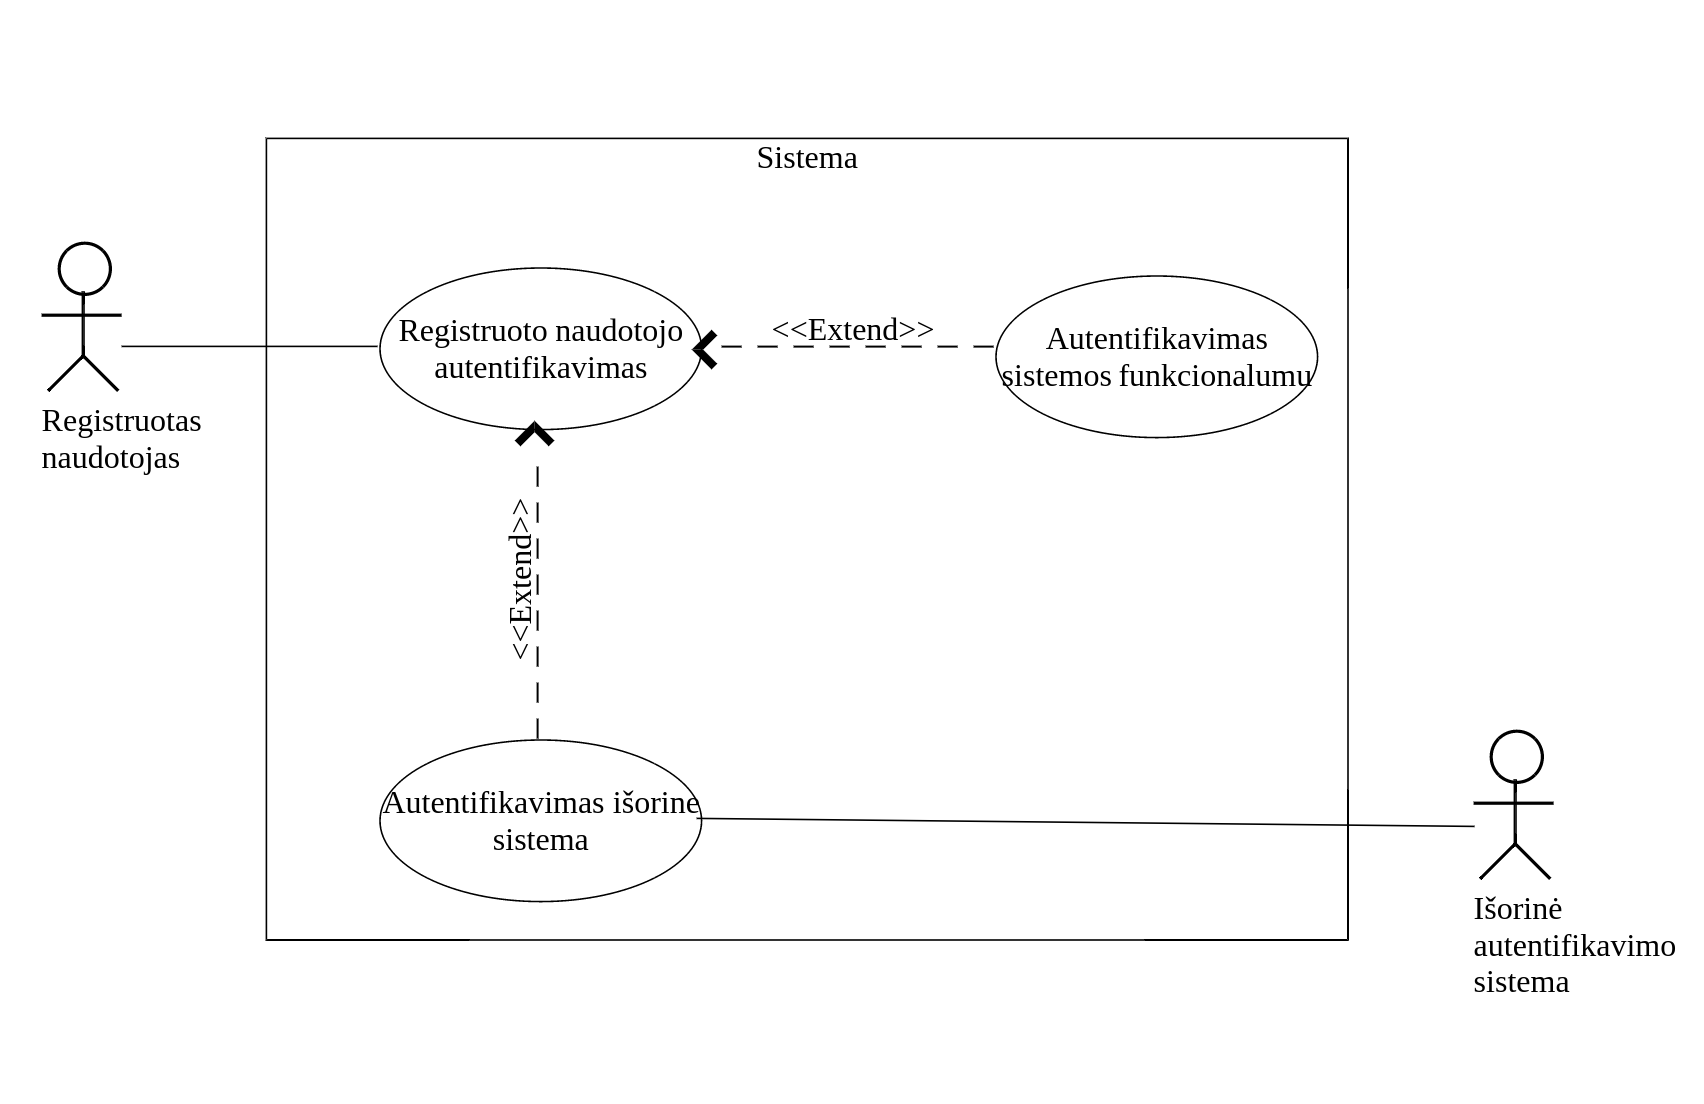
\includegraphics[height=8cm]{img/use_cases_login}
	\caption{Užduočių diagrama pagal \ref{tab:text_use_cases_login} lentelę}
	\label{img:use_cases_login}
\end{figure}

Naudojimo atvejus galima atvaizduoti užduočių diagrama. \ref{img:use_cases_login} paveikslas vaizduoja \ref{tab:text_use_cases_login} lentelėje aprašytą naudojimo atvejo užduočių diagramą. Pagrindinė užduočių seka pavaizduota naudojimo atveju „Autentifikavimasis sistemos funkcionalumu”,  alternatyvi – „Autentifikavimasis išorine sistema”, išimtinės sekos nepavaizduotos.


\subsubsection{Užduočių diagramos apimtis}
Užduočių diagrama skirta apibūdinti kaip naudotojai siekia savo tikslų pasitelkdami sistemą. Ji parodo kokie yra funkciniai reikalavimai, naudotojų taksonomiją, duomenų srautus tarp naudotojų ir sistemos. Taip pat pateikia funkcijų hierarchijos modeliavimą ir leidžia jas suskaidyti (naudojant įtraukimo ryšį). Užduočių diagrama apibūdina funkcinius reikalavimus, ji nepateikia nei funkcijų atlikimo tvarkos, nei duomenų struktūrų naudojamų sistemoje.

\subsubsection{Užduočių diagramos komponentai} \label{section:use_cases_components}
Skirtingi šaltiniai pateikia kiek skirtingus komponentus ir jų apibrėžimus. Šiame darbe daugiausia taikomi \OMG{} standartuose pateikti apibrėžimai. Toliau bus pateikiami \UML{} standarte apibrėžtos užduočių diagramos komponentai.

\begin{figure}[H]
	\centering
	
\includegraphics[height=2cm]{img/use_case_components/actor}
	\caption{Aktoriaus žymėjimo pavyzdys}
	\label{img:use_case_components_actor}
\end{figure}

Aktorius (actor) žymi naudotojo rolę. Ją gali atlikti tiek žmogus, tiek išorinė programų sistema. Aktoriai sąveikauja su bendravimo kanalais prijungtais naudojimo atvejais. Šis komponentas žymimas žmogumi iš pagaliukų (\ref{img:use_case_components_actor} pav.).

\begin{figure}[H]
	\centering
	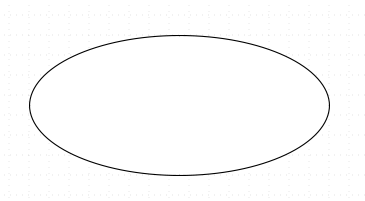
\includegraphics[height=2cm]{img/use_case_components/use_case}
	\caption{Naudojimo atvejo žymėjimo pavyzdys}
	\label{img:use_case_components_use_case}
\end{figure}

Naudojimo atvejis (use case) žymi veiklų kurias atlikus gaunamas naudingas rezultatas aibę. Rezultatas gali būti naudingas tiek vykdytojui, tiek kitiems suinteresuotiems žmonėms. Šis komponentas vaizduojamas elipse (\ref{img:use_case_components_use_case} pav.),
naudojimo atvejo pavadinimas gali būti tiek elipsėje, tiek po ja.

\begin{figure}[H]
	\centering
	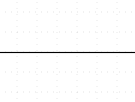
\includegraphics[width=5cm]{img/use_case_components/association}
	\caption{Bendravimo kanalo žymėjimo pavyzdys}
	\label{img:use_case_components_communication_path}
\end{figure}

Bendravimo kanalas (communication path) žymi sąveika tarp aktoriaus ir sistemos. Šis komponentas diagramoje jungia aktorių su naudojimo atveju, taip parodydamas, kad prieš atlikdamas veiklas (sistemos funkcijas) naudotojas pateikia įvestį o po jų atlikimo gaunamas rezultatas. Jeigu bendravimo kanalo ryšio su aktoriumi gausa yra daugiau nei 1 reiškia naudojimo atvejui atlikti reikalingi keli vykdytojai, jeigu bendravimo kanalo ryšio su naudojimo atveju gausa yra daugiau nei 1 reiškia aktorius gali atlikti tas pačias veiklas daugiau nei vieną kartą. Asosijacija žymima solidžia linija (\ref{img:use_case_components_communication_path} pav.).

\begin{figure}[H]
	\centering
	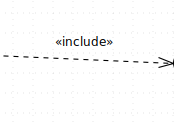
\includegraphics[height=2cm]{img/use_case_components/includes}
	\caption{Įtraukimo žymėjimo pavyzdys}
	\label{img:use_case_components_includes}
\end{figure}

Įtraukimas (includes) žymi naudojimo atvejo suskaidymą. Šis komponentas modeliuoja sąryši tarp dviejų vartojimo atvejų, taip parodydamas, kad įtraukiamo naudojimo atvejo veiklos yra atliekamos įtraukiančiame naudojimo atvejyje. Įtraukimą numatyta naudoti tuomet, kai tos pačios veiklos pasikartoja keliuose naudojimo atvejuose. Tos veiklos įdedamos į atskirą naudojimo atvejį ir prijungiamos šiuo ryšiu, tokiu būdu iškeliamas pasikartojantis funkcionalumas. Įtraukimas vaizduojamas punktyrine linija su rodykle  prie įtraukiamo naudojimo atvejo ir patikslinimu dvigubuose kampiniuose skliaustuose (\ref{img:use_case_components_includes} pav.).

\begin{figure}[H]
	\centering
	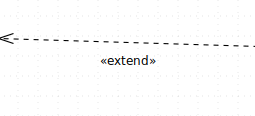
\includegraphics[height=2cm]{img/use_case_components/extend}
	\caption{Išplėtimo žymėjimo pavyzdys}
	\label{img:use_case_components_extends}
\end{figure}

Išplėtimas (extends) žymi, kad esant tam tikroms sąlygoms naudojimo atvejis įtraukia veiklas iš kitų naudojimo atvejų. Šis komponentas numatytas naudoti bendram funkcionalumui iškelti, bet kitaip nei ryšys „Įtraukia“, parodo, kad veiklos įtraukiamos ne visada. Jis vaizduojamas punktyrine linija su rodykle prie išplečiamo naudojimo atvejo ir patikslinimu dvigubuose kampiniuose skliaustuose (\ref{img:use_case_components_extends} pav.).

\begin{figure}[H]
	\centering
	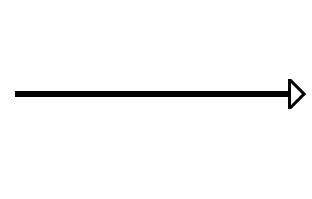
\includegraphics[height=2cm]{img/use_case_components/generalization}
	\caption{Apibendrinimo žymėjimo pavyzdys}
	\label{img:use_case_components_generalization}
\end{figure}

Apibendrinimas (generalization) žymi, kad elementas yra bendresnio elemento variantas. Nuo išplėtimo naudojimo atvejo apibendrinimas skiriasi tuo, kad pasakoma jog bent vienas iš apibendrinamų naudojimo atvejų funkcionalumų įtraukiamas į apibendrinančio naudojimo atvejo funkcionalumą. Žymimas solidžia linija su rodykle prie apibendrinamo naudojimo atvejo (\ref{img:use_case_components_generalization} pav.).

\subsubsection{Užduočių diagramos komponentų tarpusavio ryšiai}

Komponentų aprašytų \ref{section:use_cases_components} skyriuje tarpusavio ryšiai  pavaizduoti metamodeliu (\ref{img:use_cases_metamodel} pav.). Jis sudarytas pagal \UML{} ir \SysML{} standartuose pateiktą informaciją. 

\begin{figure}[H]
	\centering
	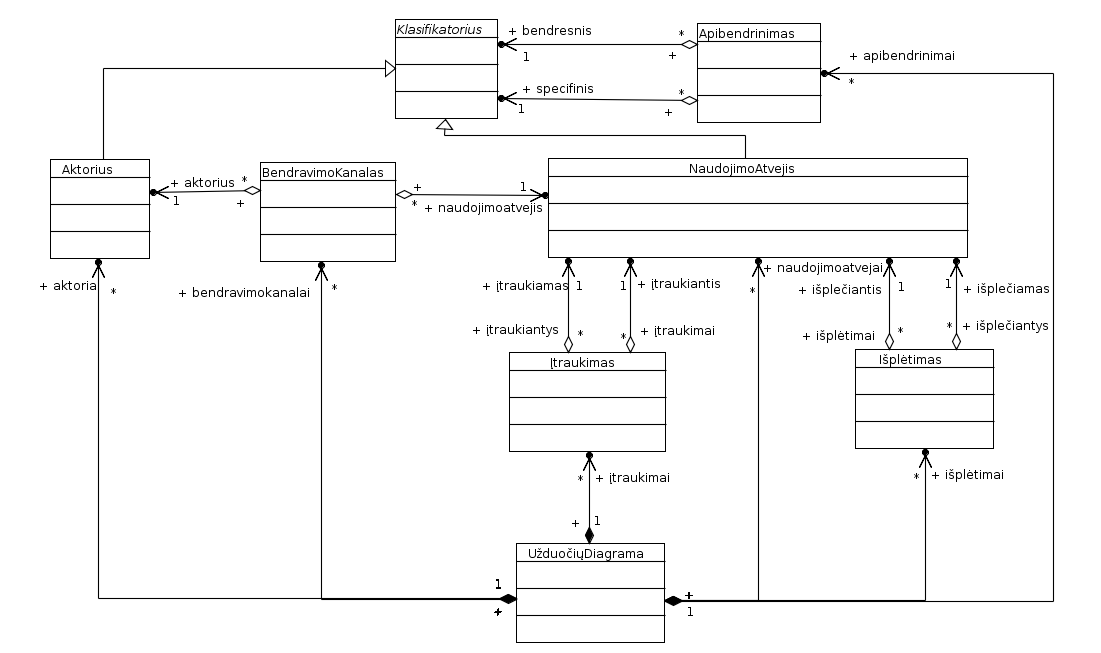
\includegraphics[width=\textwidth]{img/use_cases_metamodel}
	\caption{Užduočių diagramos metamodelis}
	\label{img:use_cases_metamodel}
\end{figure} 

Užduočių diagrama yra paketas savyje laikantis aktorius, naudojimo atvejus, bendravimo kanalus, įtraukimus, išplėtimus ir apibendrinimus. Bendravimo kanalas jungia vieną aktorių su vienu naudojimo atveju. Įtraukimas yra ryšys tarp įtraukiamo ir įtraukiančio naudojimo atvejo. Išplėtimas jungia išplečiamą naudojimo atvejį su išplečiančiu. \UML{} modelis leidžia abstraktaus tipo klasifikatoriaus apibendrinimą. Aktorius ir naudojimo atvejis yra klasifikatoriaus subtipai, todėl gali būti apibendrinti.

